\documentclass[tikz,border=7pt]{standalone}
\usepackage[scaled=0.95]{helvet}
\renewcommand{\familydefault}{\sfdefault}
\usepackage[europeanresistors,americanvoltages]{circuitikz}
\usetikzlibrary{fit,positioning,calc}
\definecolor{TEJNavy}{HTML}{1E2B55}
\definecolor{TEJBlue}{HTML}{1769AA}
\definecolor{TEJRed}{HTML}{A12622}
\begin{document}
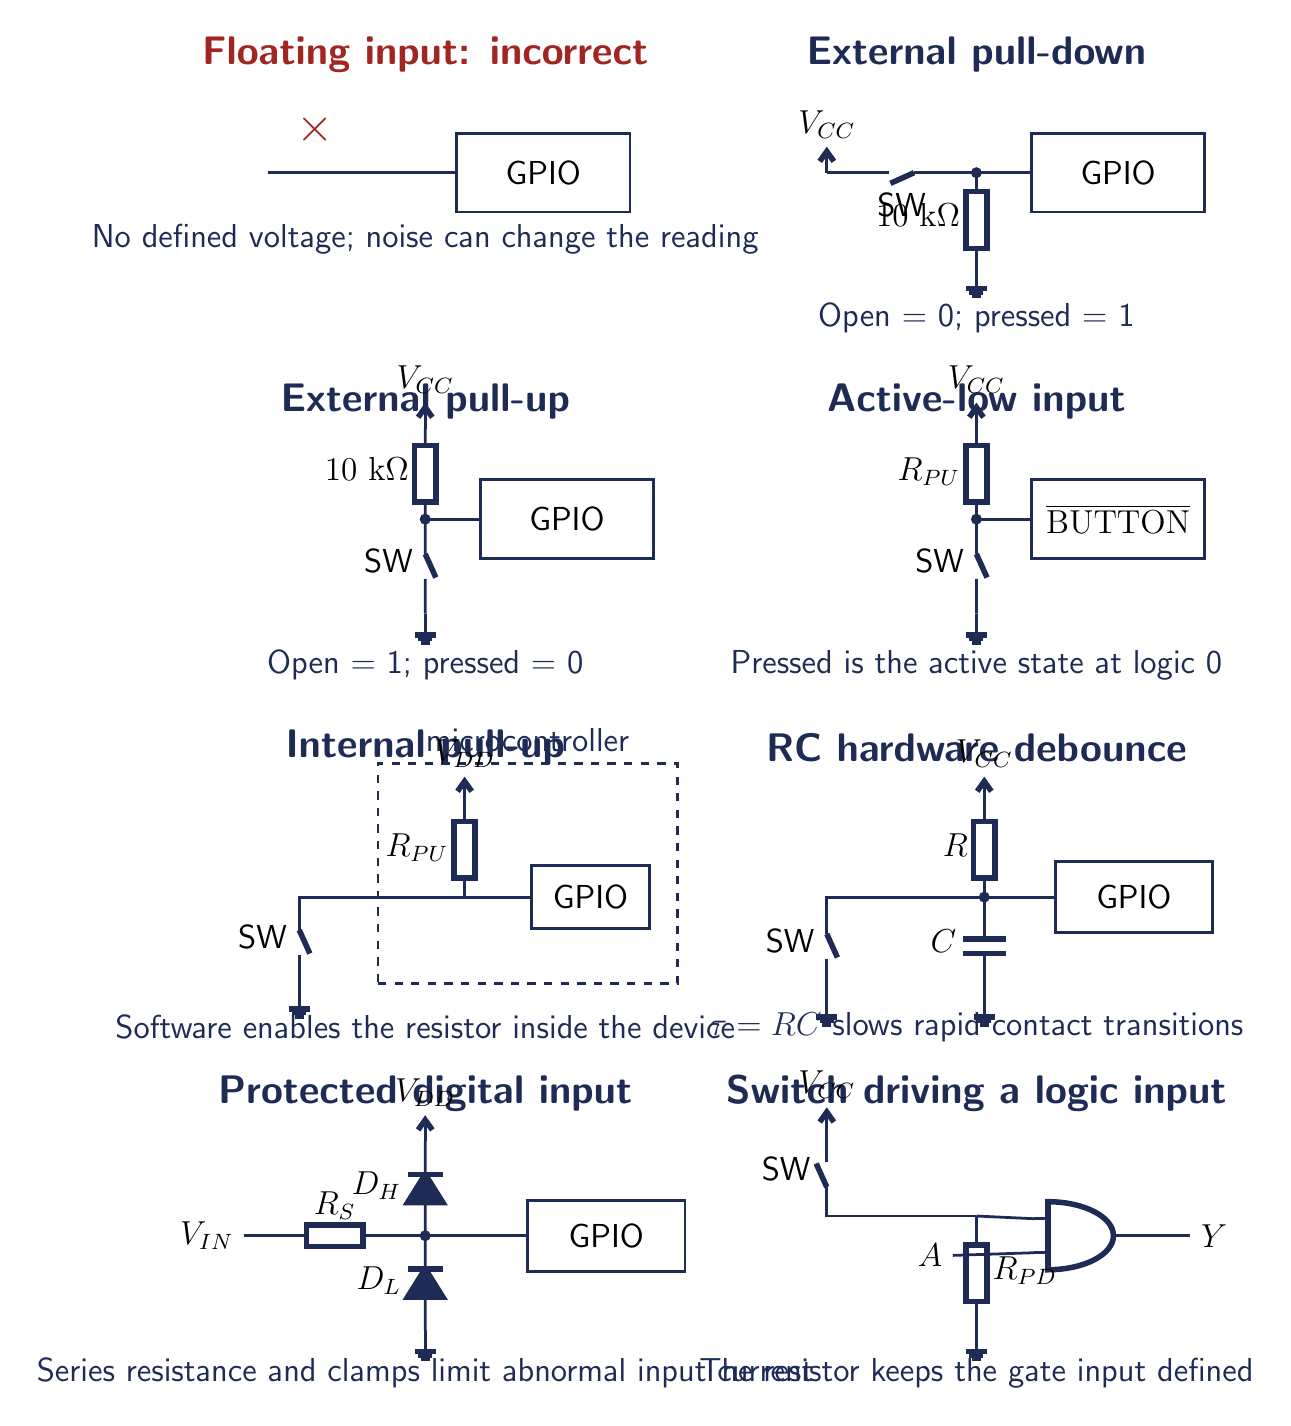
\begin{tikzpicture}[line width=1pt,draw=TEJNavy,font=\large]
  \ctikzset{bipoles/length=0.9cm}

  \begin{scope}
    \node[font=\bfseries\Large,text=TEJRed] at (2.7,7.5) {Floating input: incorrect};
    \node[draw=TEJNavy,minimum width=2.2cm,minimum height=1.0cm] (fpin) at (4.2,6.0) {GPIO};
    \draw (0.7,6.0) -- (fpin.west);
    \node[text=TEJRed,font=\bfseries\LARGE] at (1.3,6.55) {$\times$};
    \node[text=TEJNavy,align=center] at (2.7,5.15) {No defined voltage; noise can change the reading};
  \end{scope}

  \begin{scope}[xshift=7.0cm]
    \node[font=\bfseries\Large,text=TEJNavy] at (2.7,7.5) {External pull-down};
    \node[draw=TEJNavy,minimum width=2.2cm,minimum height=1.0cm] (dpin) at (4.5,6.0) {GPIO};
    \draw (2.7,6.0) -- (dpin.west);
    \draw (2.7,6.0) to[R,l_=$10\ \mathrm{k}\Omega$] (2.7,4.8) node[ground] {};
    \draw (2.7,6.0) to[nos,l=SW] (0.8,6.0) node[vcc] {$V_{CC}$};
    \fill[TEJNavy] (2.7,6.0) circle (2pt);
    \node[text=TEJNavy,align=center] at (2.7,4.15) {Open = 0; pressed = 1};
  \end{scope}

  \begin{scope}[yshift=-4.4cm]
    \node[font=\bfseries\Large,text=TEJNavy] at (2.7,7.5) {External pull-up};
    \node[draw=TEJNavy,minimum width=2.2cm,minimum height=1.0cm] (upin) at (4.5,6.0) {GPIO};
    \draw (2.7,6.0) -- (upin.west);
    \draw (2.7,6.0) to[R,l=$10\ \mathrm{k}\Omega$] (2.7,7.15) node[vcc] {$V_{CC}$};
    \draw (2.7,6.0) to[nos,l_=SW] (2.7,4.8) node[ground] {};
    \fill[TEJNavy] (2.7,6.0) circle (2pt);
    \node[text=TEJNavy,align=center] at (2.7,4.15) {Open = 1; pressed = 0};
  \end{scope}

  \begin{scope}[xshift=7.0cm,yshift=-4.4cm]
    \node[font=\bfseries\Large,text=TEJNavy] at (2.7,7.5) {Active-low input};
    \node[draw=TEJNavy,minimum width=2.2cm,minimum height=1.0cm] (alpin) at (4.5,6.0) {$\overline{\mathrm{BUTTON}}$};
    \draw (2.7,6.0) -- (alpin.west);
    \draw (2.7,6.0) to[R,l=$R_{PU}$] (2.7,7.15) node[vcc] {$V_{CC}$};
    \draw (2.7,6.0) to[nos,l_=SW] (2.7,4.8) node[ground] {};
    \fill[TEJNavy] (2.7,6.0) circle (2pt);
    \node[text=TEJNavy,align=center] at (2.7,4.15) {Pressed is the active state at logic 0};
  \end{scope}

  \begin{scope}[yshift=-8.8cm]
    \node[font=\bfseries\Large,text=TEJNavy] at (2.7,7.5) {Internal pull-up};
    \node[draw=TEJNavy,dashed,minimum width=3.8cm,minimum height=2.8cm,label={[text=TEJNavy]above:microcontroller}] (mcu) at (4.0,5.9) {};
    \node[draw=TEJNavy,minimum width=1.5cm,minimum height=0.8cm] (ipin) at (4.8,5.6) {GPIO};
    \draw (3.2,5.6) -- (ipin.west);
    \draw (3.2,5.6) to[R,l=$R_{PU}$] (3.2,6.8) node[vcc] {$V_{DD}$};
    \draw (3.2,5.6) -- (1.1,5.6) to[nos,l_=SW] (1.1,4.45) node[ground] {};
    \node[text=TEJNavy,align=center] at (2.7,3.95) {Software enables the resistor inside the device};
  \end{scope}

  \begin{scope}[xshift=7.0cm,yshift=-8.8cm]
    \node[font=\bfseries\Large,text=TEJNavy] at (2.7,7.5) {RC hardware debounce};
    \node[draw=TEJNavy,minimum width=2.0cm,minimum height=0.9cm] (rcpin) at (4.7,5.6) {GPIO};
    \draw (2.8,5.6) -- (rcpin.west);
    \draw (2.8,5.6) to[R,l=$R$] (2.8,6.8) node[vcc] {$V_{CC}$};
    \draw (2.8,5.6) to[C,l_=$C$] (2.8,4.35) node[ground] {};
    \draw (2.8,5.6) -- (0.8,5.6) to[nos,l_=SW] (0.8,4.35) node[ground] {};
    \fill[TEJNavy] (2.8,5.6) circle (2pt);
    \node[text=TEJNavy,align=center] at (2.7,3.95) {$\tau=RC$ slows rapid contact transitions};
  \end{scope}

  \begin{scope}[yshift=-13.2cm]
    \node[font=\bfseries\Large,text=TEJNavy] at (2.7,7.5) {Protected digital input};
    \node[draw=TEJNavy,minimum width=2.0cm,minimum height=0.9cm] (ppin) at (5.0,5.7) {GPIO};
    \draw (0.4,5.7) node[left] {$V_{IN}$} to[R,l=$R_S$] (2.7,5.7) -- (ppin.west);
    \draw (2.7,5.7) to[D*,l=$D_H$] (2.7,6.9) node[vcc] {$V_{DD}$};
    \draw (2.7,4.5) node[ground] {} to[D*,l=$D_L$] (2.7,5.7);
    \fill[TEJNavy] (2.7,5.7) circle (2pt);
    \node[text=TEJNavy,align=center] at (2.7,3.95) {Series resistance and clamps limit abnormal input current};
  \end{scope}

  \begin{scope}[xshift=7.0cm,yshift=-13.2cm]
    \node[font=\bfseries\Large,text=TEJNavy] at (2.7,7.5) {Switch driving a logic input};
    \node[and port,number inputs=2,scale=1.2] (gate) at (4.5,5.7) {};
    \draw (2.7,5.95) -- (gate.in 1);
    \draw (2.7,5.95) to[R,l=$R_{PD}$] (2.7,4.5) node[ground] {};
    \draw (2.7,5.95) -- (0.8,5.95) to[nos,l=SW] (0.8,7.0) node[vcc] {$V_{CC}$};
    \draw (2.4,5.45) node[left] {$A$} -- (gate.in 2);
    \draw (gate.out) -- ++(0.8,0) node[right] {$Y$};
    \node[text=TEJNavy,align=center] at (2.7,3.95) {The resistor keeps the gate input defined};
  \end{scope}
\end{tikzpicture}
\end{document}
